%!TEX root = ./intern_report.tex

\paragraph{}
I worked as a research intern at DATA61 for 24 weeks. During this time, I worked three intertwined projects under the supervision of Nicolas Hudson and Dr. Navinda Kottege. 

\paragraph{}
The first project was developing indoor-Trailnet: a classification based approach to the autonomous navigation problem. For this, first I built a robot with Uvindu Perera for data collection and testing. We designed the power distribution system of the robot and assembled a high level and low level controllers. We calculated the torque requirements for the motors, current, voltage and power limitations for the power supply components and motor controllers during this process. We learnt a lot through debugging the errors we came across and extensively troubleshooting whenever a component or circuit board is damaged to provide a report on the event. I also debugged the driver software for the motor controller and modified parts of it to fix certain issues since it was not being maintained anymore.

\begin{figure}[H]
    \centering
    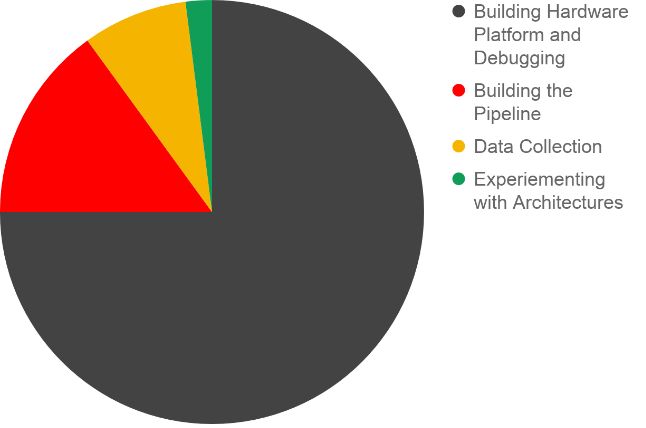
\includegraphics
        [width=9cm]
        {figures/time.PNG}
    \caption{Overview of our Time Spent}\vspace{-4mm}
\end{figure}

\paragraph{}
I learnt tensorflow and tensorflow-keras for this project and built a 20 layer residual network from scratch and trained it on the supercomputer cluster. Then I learnt tensorRT and deployed the trained network on Jetson TX2: a powerful embedded device that acted as the high level controller for the robot. I also learnt ROS (Robot Operating System) extensively, and created multiple ROS nodes and packages for testing, collecting data from sensors and for controlling the robot. 

\paragraph{}
For the next project of building an end to end pipeline for machine learning in robotics, I experimented and figured out the best practices when training models using large datasets on the supercomputer. I documented these experiments and the results, and proposed an efficient method to set up a writing and reading pipeline. I presented ~\cite{presentation} my pipeline in the Robotics Reading Group meeting. Many scientists were interested and some followed up via email asking questions and requesting to build tools for visualizing datasets.

\paragraph{}
The final project was experimental, where I explored different configurations of neural network architectures to build a robot that can climb hills while avoiding obstacles. Through literature survey and in-depth discussions with my supervisor, I learnt a lot about the structure of Deep Convolutional Neural Networks and possible methods of combining scaler data with the images to train a network. I tried several approaches here: solving the problem as a classification and a regression and using different ways to combine the inputs into the network. However, I was unable to get good results within the time we had there, due to the problems in data collection and the lack of time as we had to spend most of the time building and debugging the robot platform.

\paragraph{}
Also, I learnt about cross modal learning transfer and neural network distillation process through literature survey as a part of the project that was initially given, before we were changed into a different project a week later. Before and during the internship program, I expressed my interest in working in a project where I can develop algorithms and tackle abstract problems that could lead to new research and a publication. Unfortunately such a project was not available for interns at the time and my supervisors were satisfied with the work I was doing with hardware and deployment of machine learning. However, I learnt a lot through these projects and it had been a great experience. I also got familiarized with the software tools widely used in academia, high end sensors and controllers, and I daily worked with the Bracewell cluster, which is one of the world's largest supercomputer clusters. 

\paragraph{}
In addition to that, I learnt the etiquettes and responsibilities of working as an employee in a company. Helping others and asking for help, attending meetings and following up via official emails, documenting all the tasks and weekly progress in the wiki pages of CSIRO helped me learn a lot about these responsibilities. The work culture in DATA61 is exceptionally inclusive, where we got to work with people of multiple nationalities and share our culture. The students are allowed to work on their own pace and I was allowed to work overnight on multiple days and work on weekends as well. I also got to attend events such as DATA61 LIVE, where I could attend to many talks and discussion forums and observe the development of cutting edge technology of Australia through the exhibits.

\paragraph{}
From my experience, I would suggest DATA61 to assess the skills of the interns and assign them to projects relevant to those skills, to utilize their full potential for a project. Also, it would help if they can give an overview of the project at the beginning of the internship and set incremental goals to be completed at given deadlines. I found it disorienting when the project given to me before the internship was changed as I reached there and changed again a week later to settle on an experimental project of my supervisor that subsequently evolved into the three above projects (that I explained in Chapter 2) through the period of six months. 

\paragraph{}
I would also like to suggest NAITA to computerize the supervision process, where interns can submit the intern diary and monthly reports online. This would help because in organizations like CSIRO, the students are expected to maintain an online diary and the interns can save time by writing by hand the same thing they have typed into the online diary.

\paragraph{}
Therefore, I can conclude that my overall experience in DATA61 was great. I had the opportunity to learn a lot and make contacts. I am deeply thankful to the Industrial Training Division of our university and NAITA for this internship and I am thankful for DATA61 and my supervisors for providing me with such an exceptional opportunity and a training experience.





